\section{心得}

這次卡最久的是透視投影的參數。\lstinline|glFrustum| 要給 near 平面的上下左右邊界，我一開始直接填數字，怎麼調畫面都不對，不是被拉長就是看到的範圍怪怪的。
後來上網查，在論壇看到有人用 tan 從視角算邊界：
\[
    \text{top} = \text{near} \cdot \tan\frac{\text{fovY}}{2}, \qquad
    \text{right} = \text{top} \cdot \text{aspect}
\]
照這樣算之後畫面就正常了，視窗大小改變時比例也不會跑掉。

此外，我也亂嘗試了一下，故意先呼叫 \lstinline|glOrtho| 再呼叫 \lstinline|glFrustum|，讓兩個矩陣乘在一起，就得到圖~\ref{fig:ortho-frustum} 這個很神奇的畫面。

\begin{figure}[htbp]
    \centering
    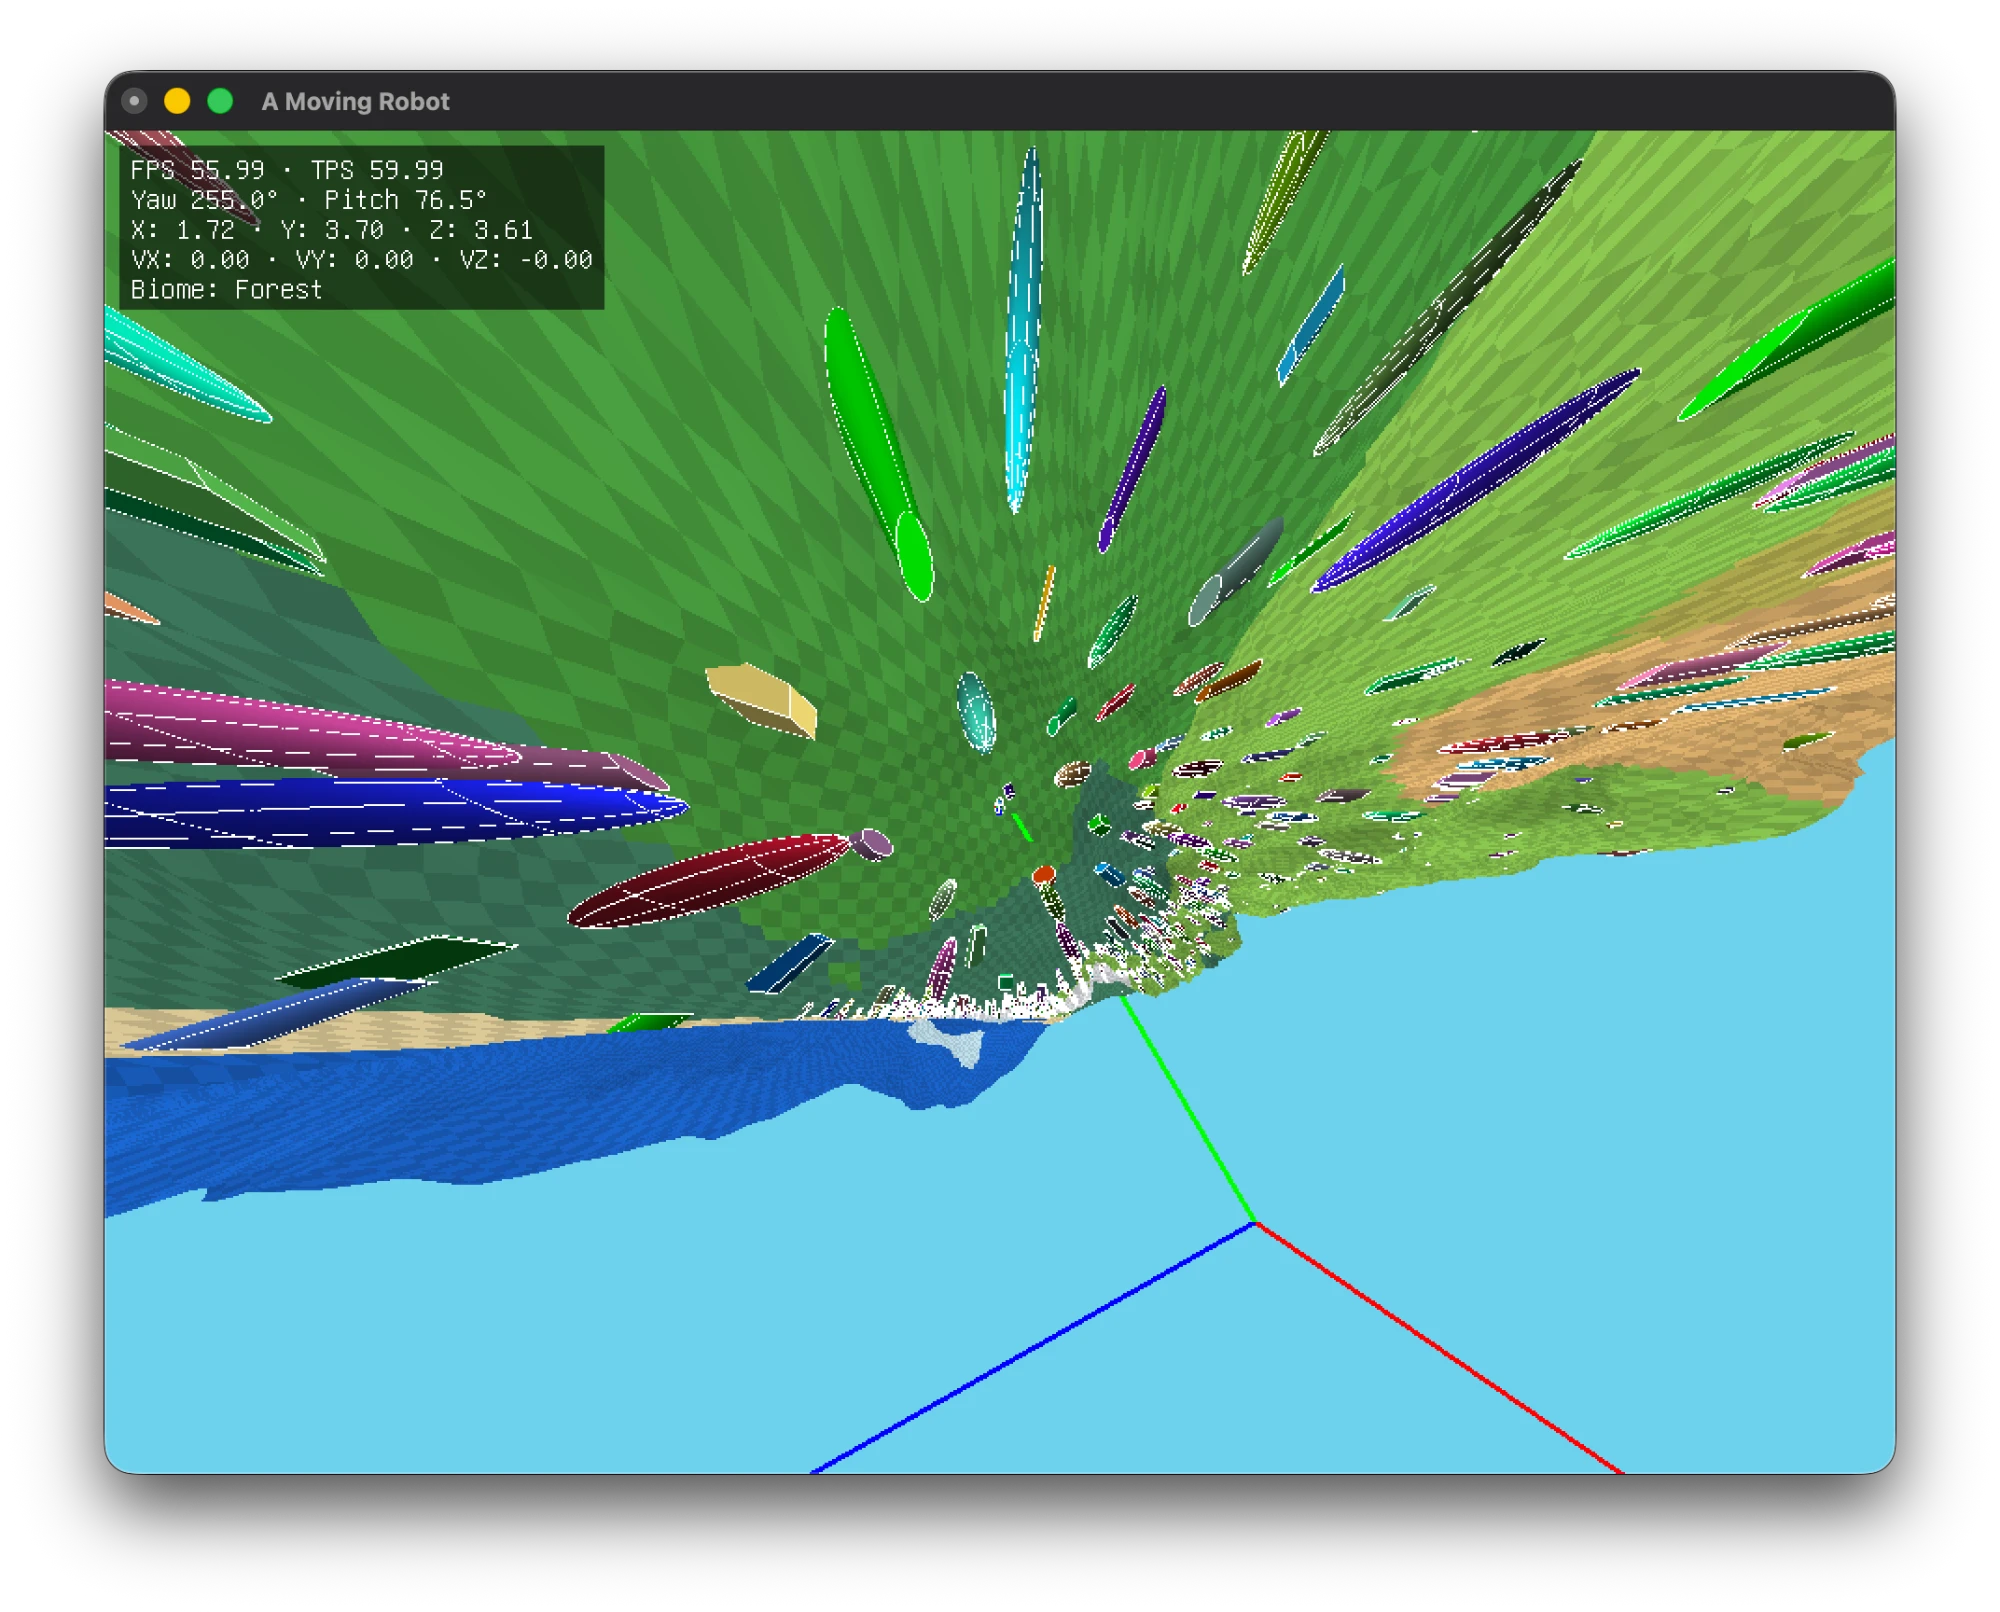
\includegraphics[width=.45\textwidth]{docs/figures/hw3/ortho-times-frustum.png}
    \caption{\lstinline|glOrtho| 與 \lstinline|glFrustum| 疊在一起的投影}
    \label{fig:ortho-frustum}
\end{figure}
